\section{PHƯƠNG TRÌNH QUY VỀ PHƯƠNG TRÌNH BẬC HAI}

\subsection{LÝ THUYẾT CẦN NHỚ}
\subsubsection{Giải phương trình dạng $\sqrt{ax^2+bx+c}=\sqrt{dx^2+ex+f}$}
\indamm{Phương pháp giải:}
\begin{itemize}
	\item [$\bullet$] Bình phương hai vế của phương trình (làm mất căn thức ), ta được
	$$ax^2+bx+c=dx^2+ex+f$$
	\textit{Chuyển vế, thu gọn ta được phương trình bậc hai. Giải phương trình này, tìm nghiệm.}
	\item [$\bullet$] Thay từng nghiệm vừa tìm được vào phương trình ban đầu. Nghiệm nào thoả mãn thì nhận; nghiệm nào \textbf{không} thoả thì loại.
	\item [$\bullet$] Kết luận nghiệm của phương trình đã cho.
\end{itemize}
\subsubsection{Giải phương trình dạng $\sqrt{ax^2+bx+c}=dx+e$}
\indamm{Phương pháp giải:}
\begin{itemize}
	\item [$\bullet$] Bình phương hai vế của phương trình (làm mất căn thức ), ta được
	$$ax^2+bx+c=(dx+e)^2$$
	\textit{Chuyển vế, thu gọn ta được phương trình bậc hai. Giải phương trình này, tìm nghiệm.}
	\item [$\bullet$] Thay từng nghiệm vừa tìm được vào phương trình ban đầu. Nghiệm nào thoả mãn thì nhận; nghiệm nào \textbf{không} thoả thì loại.
	\item [$\bullet$] Kết luận nghiệm của phương trình đã cho.
\end{itemize}

\subsection{RÈN LUYỆN KĨ NĂNG GIẢI TOÁN}
\begin{dang}{Giải phương trình dạng $\sqrt{ax^2+bx+c}=\sqrt{dx^2+ex+f}$}
\begin{listEX}[1]
	\item [\ding{172}] \indamm{Phương pháp giải:} Bình phương hai vế, giải tìm $x$. Sau đó, thử lại và chọn nghiệm.
	\item [\ding{173}] \indamm{Chú ý:} 
	\begin{enumEX}[$\bullet$]{2}
		\item $(a+b)^2=a^2+2ab+b^2$.
		\item $(a-b)^2=a^2-2ab+b^2$.
	\end{enumEX}
\end{listEX}
\end{dang}

\begin{vd}
	Giải các phương trình sau:
	\begin{enumEX}[a)]{2}
		\item $\sqrt{5 x^{2}-28 x-29}=\sqrt{x^{2}-5 x+6}$;
		\item $\sqrt{6 x^{2}-22 x+14}=\sqrt{4 x^{2}-11 x-1}$;
		\item $\sqrt{-x^{2}+x+17}=\sqrt{x^{2}-12 x+2}$;
		\item $\sqrt{x^2-6x-4}=\sqrt{x-4}$.
		\item $\sqrt{2x^2+3x+1}-\sqrt{x^2+4x+3}=0$.
		\item $\sqrt{2x^2+3x-2}-\sqrt{x^2+x+6}=0$;
	\end{enumEX}
\loigiai{
\begin{enumerate}[a)]
	\item Bình phương hai vế của phương trình đã cho, ta được
	$$
	\begin{aligned}
		& 5 x^{2}-28 x-29=x^{2}-5 x+6 \\
		\Rightarrow & 4 x^{2}-23 x-35=0 \\
		\Rightarrow & x=7 \text { hoặc } x=-\dfrac{5}{4} .
	\end{aligned}
	$$
	Thay lần lượt các giá trị trên vào phương trình đã cho, ta thấy $x=7$ và $x=-\dfrac{5}{4}$ thoả mãn.
	Vậy nghiệm của phương trình đã cho là $7$ và $-\dfrac{5}{4}$.
	\item Bình phương hai vế của phương trình đã cho, ta được
	$$
	\begin{aligned}
		& 6 x^{2}-22 x+14=4 x^{2}-11 x-1 \\
		\Rightarrow & 2 x^{2}-11 x+15=0 \\
		\Rightarrow & x=\dfrac{5}{2} \text { hoặc } x=3
	\end{aligned}
	$$
	Thay lần lượt các giá trị trên vào phương trình đã cho, ta thấy chỉ có $x=3$ thoả mãn.
	Vậy nghiệm của phương trình đã cho là $x=3$.
	\item Bình phương hai vế của phương trình đã cho, ta được
	$$
	\begin{aligned}
		&-x^{2}+x+17=x^{2}-12 x+2 \\
		\Rightarrow &-2 x^{2}+13 x+15=0 \\
		\Rightarrow & x=-1 \text { hoặc } x=\dfrac{15}{2} .
	\end{aligned}
	$$
	Thay lần lượt các giá trị trên vào phương trình đã cho, ta thấy chỉ có $x=-1$ thoả mãn.
	Vậy nghiệm của phương trinh đã cho là $x=-1$.
	\item Bình phương hai vế của (1) ta được $x^2-6x-4=x-4$. \hfill (2)\\
	Ta có $(2)\Leftrightarrow x^2-7x=0$.\\
	Do đó, phương trình (2) có hai nghiệm là $x=0$ và $x=7$.\\
	Thay lần lượt hai giá trị trên vào bất phương trình $x-4\geq 0$, ta thấy chỉ có $x=7$ thoả mãn bất phương trình.\\
	Vậy nghiệm của phương trình (1) là $x=7$.
	\item Chuyển vế ta được $\sqrt{2x^2+3x+1}=\sqrt{x^2+4x+3}$.\\
	Bình phương hai vế của (3) ta được $2x^2+3x+1=x^2+4x+3$. \hfill (4)\\
	Ta có $(4)\Leftrightarrow x^2-x-2=0$.\\
	Do đó, phương trình (4) có hai nghiệm là $x=-1$ và $x=2$.\\
	Thay lần lượt hai giá trị trên vào bất phương trình $x^2+4x+3\geq 0$, ta thấy cả hai giá trị đều thoả mãn bất phương trình.\\
	Vậy phương trình(3) có hai nghiệm là $x=-1$ và $x=2$.
	\item Ta có
	\begin{eqnarray*}
		&& \sqrt{2x^2+3x-2}=\sqrt{x^2+x+6}\Leftrightarrow \heva{&x^2+x+6\geq 0\\&2x^2+3x-2=x^2+x+6}\\
		&\Leftrightarrow & \heva{&\forall x\in \mathbb{R}\\&x^2+2x-8=0}\Leftrightarrow  \heva{&\forall x\in \mathbb{R}\\&\hoac{&x=2\\&x=-4}}\Leftrightarrow \hoac{&x=2\\&x=-4.}
	\end{eqnarray*}
	Vậy, phương trình có nghiệm $x=2$ hoặc $x=-4$.
\end{enumerate}}
\end{vd}
\dongcham{42}
\begin{dang}{Giải phương trình dạng $\sqrt{ax^2+bx+c}=dx+e$}
\begin{listEX}[1]
	\item [\ding{172}] \indamm{Phương pháp giải:} Bình phương hai vế, giải tìm $x$. Sau đó, thử lại và chọn nghiệm.
	\item [\ding{173}] \indamm{Chú ý:} 
	\begin{enumEX}[$\bullet$]{2}
		\item $(a+b)^2=a^2+2ab+b^2$.
		\item $(a-b)^2=a^2-2ab+b^2$.
	\end{enumEX}
\end{listEX}
\end{dang}

\begin{vd}
	Giải các phương trình sau:
	\begin{enumEX}[a)]{2}
		\item $\sqrt{2x^2+3x-1}=x+3$;
		\item $\sqrt{2x^2-3x-1}=3x+5$;
		\item $\sqrt{69 x^{2}-52 x+4}=-6 x+4$;
		\item $\sqrt{-x^{2}-4 x+22}=-2 x+5$;
		\item $\sqrt{-7 x^{2}-60 x+27}+3(x-1)=0$;
		\item $\sqrt{3 x^{2}-9 x-5}+2 x=5$.
	\end{enumEX}
\loigiai{
	\begin{enumerate}[a)]
		\item Bình phương hai vế ta được $2x^2+3x-1=(x+3)^2 \Leftrightarrow x^2 -3x - 10 = 0 \Leftrightarrow x=-2$ hoặc $x=5$.\\
		Thử lại,  hai giá trị này đều thỏa phương trình ban đầu. Suy ra $S=\{-2;5\}$.
		\item Bình phương hai vế ta được $2x^2-3x-1=(3x+5)^2 \Leftrightarrow -7x^2 -33x - 26 = 0 \Leftrightarrow x=-1$ hoặc $x=-\dfrac{26}{7}$.\\
		Thử lại,  chỉ có $x=-1$ thỏa phương trình ban đầu. Suy ra $S=\{-1\}$.
		\item
		\item 
		\item 
		\item Ta có: $\quad \sqrt{3 x^{2}-9 x-5}+2 x=5$
		$$
		\Rightarrow \sqrt{3 x^{2}-9 x-5}=5-2 x
		$$
		Bình phương hai vế của phương trình (1), ta được:
		$$
		\begin{aligned}
			& 3 x^{2}-9 x-5=(-2 x+5)^{2} \\
			\Rightarrow & 3 x^{2}-9 x-5=4 x^{2}-20 x+25 \\
			\Rightarrow &-x^{2}+11 x-30=0
		\end{aligned}
		$$
		$$
		\Rightarrow x=5 \text { hoặc } x=6 \text {. }
		$$
		Thay lần lượt các giá trị trên vào phương trình đã cho, ta thấy $x=5$ và $x=6$ không thoả mãn.
		Vậy phương trình vô nghiệm.
\end{enumerate}}
\end{vd}
\dongcham{31}
\begin{dang}{Vận dụng, thực tiễn}
\end{dang}
\begin{vd}
	\immini{Khoảng cách từ nhà An ở vị trí $N$ đến cột điện $C$ là $10 \mathrm{~m}$. Từ nhà, An đi $x$ mét theo phương tạo với $NC$ một góc $60^{\circ}$ đến vị trí $A$ sau đó đi tiếp $3 \mathrm{~m}$ đến vị trí $B$ như hình bên.
		\begin{tasks}(1)
			\task Biểu diễn khoảng cách $AC$ và $BC$ theo $x$.
			\task Tìm $x$ để $A C=\dfrac{8}{9} BC$.
			\task Tìm $x$ đề khoảng cách $BC=2 AN$.
		\end{tasks}
	\textit{Lưu ý: Đáp số làm tròn đến hàng phần mười.}}{
	\begin{tikzpicture}[smooth,scale=1.2]
		\path
		(0,0) coordinate (N)
		(3,0) coordinate (C)
		($(N)!1.2!60:(C)$) coordinate (B)
		($(B)!0.3!(N)$) coordinate (A)
		;
		\draw (N)--(C)--(B)--cycle (C)--(A)
		pic[draw, angle radius=4mm]{angle=C--N--B}
		pic["\scriptsize $60^\circ$",angle radius=13mm]{angle=C--N--B}
		;
		\path 
		(N)--(A) node[left,midway,scale=.8]{$x$ }
		(A)--(B) node[above,midway,sloped,scale=.8]{$3$ }
		(N)--(C) node[above,midway,sloped,scale=.8]{$10$ }
		;
		\foreach \x/\g in {A/-160,N/-90,C/-90,B/90} \draw[fill=black] (\x) circle (.05) +(\g:.3) node{$\x$};
\end{tikzpicture}}
\loigiai{
	\begin{enumerate}[a)]
		\item Vì $x$ là khoảng cách $AN$ nên $x \geq 0$.
		$$
		\begin{aligned}
			A C=\sqrt{A N^{2}+N C^{2}-2 A N \cdot N C \cdot \cos 60^{\circ}} &=\sqrt{x^{2}+100-10 x} \\
			B C=\sqrt{B N^{2}+N C^{2}-2 B N \cdot N C \cdot \cos 60^{\circ}} &=\sqrt{(x+3)^{2}+100-10(x+3)} \\
			&=\sqrt{x^{2}-4 x+79} .
		\end{aligned}
		$$
		\item Ta có $A C=\dfrac{8}{9} B C$
		$$
		\begin{aligned}
			&\Rightarrow \sqrt{x^{2}-10 x+100}=\dfrac{8}{9} \sqrt{x^{2}-4 x+79} \\
			&\Rightarrow 81\left(x^{2}-10 x+100\right)=64\left(x^{2}-4 x+79\right) \\
			&\Rightarrow 17 x^{2}-554 x+3044=0 \\
			&\Rightarrow x \approx 25,6 \text { hoặc } x \approx 7
		\end{aligned}
		$$
		Vậy $x \approx 25,6$ hoặc $x \approx 7$.
		\item Ta có $B C=2 A N$
		$$
		\begin{aligned}
			&\Rightarrow \sqrt{x^{2}-4 x+79}=2 x \\
			&\Rightarrow x^{2}-4 x+79=4 x^{2} \\
			&\Rightarrow 3 x^{2}+4 x-79=0 \\
			&\Rightarrow x \approx 4,5 \text { hoặc } x \approx-5,8
		\end{aligned}
		$$
		Mà vì $x \geq 0$ nên ta có $x \approx 4,5$.
\end{enumerate}}
\end{vd}
\dongcham{18}
\begin{vd}
	\immini{Mặt cắt đứng của cột cây số trên quốc lộ có dạng nửa hình tròn ở phía trên và phía dưới có dạng hình chữ nhật (xem hình bên). Biết rằng đường kính của nửa hình tròn cüng là cạnh phía trên của hình chữ nhật và đường chéo của hình chữ nhật có độ dài $66 \mathrm{~cm}$. Tìm kích thước của hình chữ nhật, biết rằng diện tích của phần nửa hình tròn bằng 0,3 lần diện tích của phần hình chữ nhật. Lấy $\pi=3,14$ và làm tròn kết quả đến chữ số thập phân thứ hai.}{\hspace{1cm}
	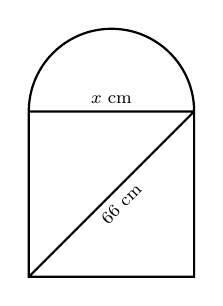
\begin{tikzpicture}[smooth,font=\footnotesize,scale=0.7,thick]
		\path
		(0,0) coordinate (O)
		(-1.5,0) coordinate (A)
		(1.5,0) coordinate (B)
		(1.5,-3) coordinate (C)
		(-1.5,-3) coordinate (D)
		;
		\draw 
		(A)--(B)--(C)--(D)--cycle
		(D)--(B)
		(0:1.5 cm) arc (0:180:1.5 cm);
		\path 
		(D)--(B) node[below,midway,sloped,scale=.8]{$66$ cm }
		(B)--(A) node[above,midway,scale=.8]{$x$ cm }
		;
	
\end{tikzpicture}}
	\loigiai{
	Gọi đường kính của nửa hình tròn là $x(\mathrm{~cm})(x>0)$. Độ dài cạnh bên của hình chữ nhật là $\sqrt{66^{2}-x^{2}}$. Diện tích nửa hình tròn là $\frac{3,14 x^{2}}{8}$. Diện tích hình chữ nhật là $x \sqrt{66^{2}-x^{2}}$. Theo giả thiết ta có:
	$$
	\begin{aligned}
		\dfrac{3,14 x^{2}}{8}=0,3 x \sqrt{66^{2}-x^{2}} & \Leftrightarrow 157 x=120 \sqrt{66^{2}-x^{2}} \\
		& \Leftrightarrow x^{2}=\dfrac{62726400}{39049} \Leftrightarrow x \approx \pm 40,08 .
	\end{aligned}
	$$
	Vậy kích thước của hình chữ nhật khoảng $40,08 \mathrm{~cm} \times 52,44 \mathrm{~cm}$.}
\end{vd}
\dongcham{18}
\begin{vd}
	\immini{Một công ty muốn làm một đường ống dẫn từ một điểm $A$ trên bờ đến một điểm $C$ trên một hòn đảo. Hòn đảo cách bờ biển $6 \mathrm{~km}$. Để thực hiện, công ty dự định xây dựng phần đường ống trên bờ từ A đến B và đường ống dưới nước từ B đến C (hình vẽ).  Biết giá để xây đường ống trên bờ là $50.000 \mathrm{USD}$ mỗi km, và $130.000 \mathrm{USD}$ mỗi km để xây dưới nước. Xác định đoạn đường từ $A$ đến $B$ để tổng chi phí xây dựng lăp đặt từ A đến C khoảng 1.170.000 USD.}{
	\begin{tikzpicture}[scale=0.22, font=\footnotesize, line join=round, line cap=round, >=stealth]
		\def\m{1}
		\begin{scope}%[opacity=0.75]
			\clip(-30,10)rectangle(10,-10);
			\fill[cyan!20,,opacity=0.5](-30,10)rectangle(10,-10);
			\fill[orange!30!brown,opacity=0.5](-30,0)rectangle(10,-10);
			\fill [left color=brown!60!green,right color=brown!30!orange,line width=1.5pt,->,decorate,
			decoration={snake,amplitude=0.5mm,segment length=0.5 cm,post length=0.5 mm}](-10,0)..controls++(20:5) and++(-140:2)..(0,3)..controls++(-70:2) and++(170:3)..(10,0)--cycle;
			\tikzset{co/.pic={
					\fill[green!80!teal,out=110,in=-20] (0,0)to(-1,1)[out=-10,in=120]to(-0.2,0.7)[out=110,in=-20]to(0,1.5)[out=-40,in=100]to(0.5,0.5)[out=40,in=-120]to(1,1.3)--(0.75,0)--cycle;
			}}
			\foreach \x/\y [count=\i]in{-3/0.2,-5/0.7,5/0.2,3/0.4,0/1.2,-8/0,-2/2}
			\path(\x,\y)pic[xslant=\i/30,yscale=\i/5]{co};
			\fill [cyan,decorate,
			decoration={snake,amplitude=0.5mm,segment length=1 cm,post length=0.5 mm},,opacity=0.5]
			(-40,0.25)--++(80,0)--++(-90:5)..controls++(-140:10) and++(-150:5)..(-20,-5)--cycle;
			\tikzset{Icon-mattroi/.pic={
					\def\r{0.35}
					\fill(0,0)circle(\r);
					\draw[line width=2*\r pt](0,0)circle(\r);
					\foreach \g in{1,...,10}{
						\draw[line width=5 pt](\g*36:1.2*\r)++(\g*36:0.1*\r)--++(\g*36:\r*0.25);
					}
			}}
			%%Mây
			\tikzset{Icon-may/.pic={
					\def\r{0.35}
					\fill[white,line width=2.5*\r pt](-\r,0)--(\r,0)..controls++(0:\r) and ++(30:\r)..(0.8*\r,\r)..controls++(100:\r) and ++(80:\r)..(-0.75*\r,0.8*\r)..controls++(140:\r) and++(180:\r)..(-\r,0);
			}}
			%%Hết mây
			
			\draw[line width=3pt,orange](6,0.5)coordinate(C)--++(-120:10)coordinate(B)--++(180:15)coordinate(A)($(A)!(C)!(B)$)coordinate(H);
			\draw[dashed](C)--(H)node[pos=0.5,right]{$6$ km}--(B);
		\end{scope}
		\foreach \d/\g in{C/90,H/0,B/110,A/180}
		\draw[fill=black](\d)circle(1pt)node[shift={(\g:0.5)}]{$\d$};
		\draw[<->,dashed]([shift={(0,-1)}]A)--([shift={(0,-1)}]H)node[below,pos=0.6]{$9$ km};
\end{tikzpicture}}
	 \loigiai{
	 Đặt $x=BH$, $x \in[0 ; 9]$. Khi đó
	 $$
	 BC=\sqrt{x^2+36};\, AB=9-x
	 $$
	 Chi phí xây dựng đường ống là
	 $$
	 C(x)=130.000 \sqrt{x^{2}+36}+50.000(9-x)
	 $$
	 Để chi phí khoảng 1.170.000, ta có phương trình
	 $$130.000 \sqrt{x^{2}+36}+50.000(9-x)=1.170.000 \Leftrightarrow x=\dfrac{5}{2}$$
	 Suy ra $AB=9-x=6,5$ km.}
\end{vd}
\dongcham{18}

\begin{vd}
	\immini{Cho tứ giác $ABCD$ có $AB \perp CD$ ; $AB=2$ ; $BC=13$ ; $CD=8$ ; $DA=5$. Gọi $H$ là giao điểm của $A B$ và $CD$ và đặt $x=AH$. Hãy thiết lập một phương trình để tính độ dài $x$, từ đó tính diện tích tứ giác $ABCD$.}{
		\begin{tikzpicture}[smooth,font=\footnotesize,scale=0.9]
			\path
			(0,0) coordinate (H)
			(7,0) coordinate (C)
			(0,-4) coordinate (B)
			($(H)!0.35!(C)$)coordinate (D)
			($(H)!0.7!(B)$)coordinate (A)
			;
			\draw[thick] (A)--(D)--(C)--(B)--cycle
			;
			\draw[dashed] (A)--(H)--(D);
			\foreach \x/\g in {H/120,D/90,C/90,B/180,A/180} \draw [fill=black] (\x) circle (.05) + (\g:.45) node{$\x$};
			\path 
			(A)--(H) node[left,midway,scale=.8]{$x$ }
			(B)--(A) node[left,midway,scale=.7]{$2$ }
			(B)--(C) node[below,midway,sloped,scale=.8]{$13$ }
			(D)--(C) node[above,midway,scale=.7]{$8$ }
			(A)--(D) node[left,midway,scale=.8]{$5$ }
			;
	\end{tikzpicture}}
	\loigiai{
		Đặt $A H=x$. Khi đó theo định lí Pythagore, ta có $D H=\sqrt{25-x^2}$.
		Từ $BH^2+CH^2=BC^2$, biến đổi và rút gọn hệ thức này ta được phương trình
		$$
		4 \sqrt{25-x^{2}}=19-x
		$$
		Giải phương trình này ta được nghiệm $x=3$.
		Từ đây ta tính được $S_{ABCD}=S_{HBC}-S_{HAD}=30-6=24$ (đvdt).
	}
\end{vd}
\dongcham{18}



